\documentclass[11pt, a4paper, english]{article}
\usepackage{babel}
\usepackage{fontspec}
\usepackage{libertinus}%
\usepackage{float}
\usepackage{parskip}
\usepackage[version=4]{mhchem}
\usepackage[figuresleft]{rotating}
\usepackage{graphicx}
\usepackage{amsmath}
\usepackage{slashed}
\usepackage{fancyhdr} 
\usepackage[dvipsnames, table]{xcolor}
\usepackage{wrapfig}
\usepackage[labelfont=bf, skip=4pt, figureposition=bottom, font=normalsize]{caption}
\usepackage{siunitx}
\usepackage{adjustbox}
\usepackage{booktabs} 
\usepackage{multirow}
\usepackage[a4paper,left=2cm,right=2cm,top=2.5cm,bottom=2.5cm]{geometry}
\usepackage{csquotes}
\usepackage{enumitem}
\usepackage{subcaption}
\usepackage{listings}
\usepackage{abstract}
\usepackage{hyperref} 
%%adapted to Galician (GZ)
%\renewcommand{\tableautorefname}{Cadro}
\usepackage{lipsum}

%% ENUMITEM settings
%\setlist{itemsep=4pt}
\setlist[enumerate,1]{
	label={\bfseries \arabic*.},
}

%% SIUNITX
%\sisetup{output-decimal-marker = {,}}
\sisetup{exponent-product= \cdot}
\sisetup{separate-uncertainty=false}
\sisetup{table-parse-only=true}
\sisetup{inter-unit-product = \ensuremath { { } \cdot { } } }
\sisetup{detect-all}
\sisetup{group-digits=integer}
\sisetup{print-unity-mantissa=false}
\sisetup{list-final-separator = { e }}
\sisetup{range-phrase = -}
\sisetup{range-units = single}
\sisetup{list-units = single}
\sisetup{propagate-math-font = true}
\sisetup{text-series-to-math = true}
\sisetup{list-final-separator = { e }}
\sisetup{list-pair-separator = { e }}
\DeclareSIUnit{\espesor}{\milli\g\per\cm\squared}
\DeclareSIUnit{\aten}{\cm\squared\per\milli\g}
\DeclareSIUnit\clight{\text{\ensuremath{c}}}
\DeclareSIUnit\year{a}
\DeclareSIUnit{\barn}{b}
\DeclareSIUnit{\bar}{bar}
\DeclareSIUnit{\neutrons}{\text{neutróns}}
\DeclareSIUnit{\deuterons}{\text{deuteróns}}
\DeclareSIUnit{\counts}{\text{contas}}

%%OTHER COMMANDS
%% for isotopes
\newcommand{\iso}[2]{\ce{^{#1}#2}}
%for vectors
\newcommand{\vect}[1]{\boldsymbol{#1}}
%for ann
\newcommand{\ann}{a_{nn}}
% figure sizes
\newcommand*{\fw}{0.6}
%%for the listing package
\definecolor{backcolour}{rgb}{0.95,0.95,0.92}
\lstset{
	%backgroundcolor=\color{backcolour},
	basicstyle=\normalsize\ttfamily,
	language=C++,
	keepspaces=false,
	keywordstyle=\bfseries\color{BurntOrange},
	morekeywords={VCluster, VFilter, TPCData, std, tuple, Point, Vector, MEventReduced,
	SilData, ModularData, MergerData},
	stringstyle=\color{Orange},
	identifierstyle=\color{ProcessBlue},
	breaklines=false,
	captionpos=b,
	% belowskip=-0.85 \baselineskip,
	%columns=flexible,
}

\title{\textbf{\textit{ActRoot} manual}}
\author{Miguel Lozano González\\
	% \small{Prácticas optativas de Grao $\cdot$ Curso 22-23}\\
	% \small{Universidade de Santiago de Compostela}
	}
\date{\empty}%\date{\today}

\pagestyle{fancy}
\fancyhf{}
%\fancyhead[R]{\thepage}
\fancyhead[R]{\textsc{actroot manual}}
\fancyfoot[C]{\thepage}
\renewcommand{\headrulewidth}{0.75pt}
%\renewcommand{\footrulewidth}{0.75pt}
\setlength{\headheight}{14.5pt}

\hypersetup{
	colorlinks=true,
	linkcolor=blue,
	filecolor=magenta,      
	urlcolor=cyan,
}

%% BIBLIOGRAPHY
\usepackage[
backend=biber,
style=numeric,
sorting=none
]{biblatex}
\addbibresource{./biblio.bib}

%% DOCUMENT

\begin{document}
\begin{minipage}{0.48\linewidth}
	\maketitle
\end{minipage}\hfill
\begin{minipage}{0.48\linewidth}
	\tableofcontents
\end{minipage}

\noindent\rule{\textwidth}{1pt}

\section{Introduction}
\textit{ActRoot} aims at being a simple program to convert, process, and obtain the physical data for an ACTAR TPC experiment. It follows the structure of \textit{NPTools}\cite{nptools}, creating different \textit{detector} classes that perform custom tasks on each component of the experiment. A range of different data classes stores meaningful information at all stages of the analysis.

The following picture depicts a simplified scheme of the code.
\begin{figure}[htbp]
	\centering
	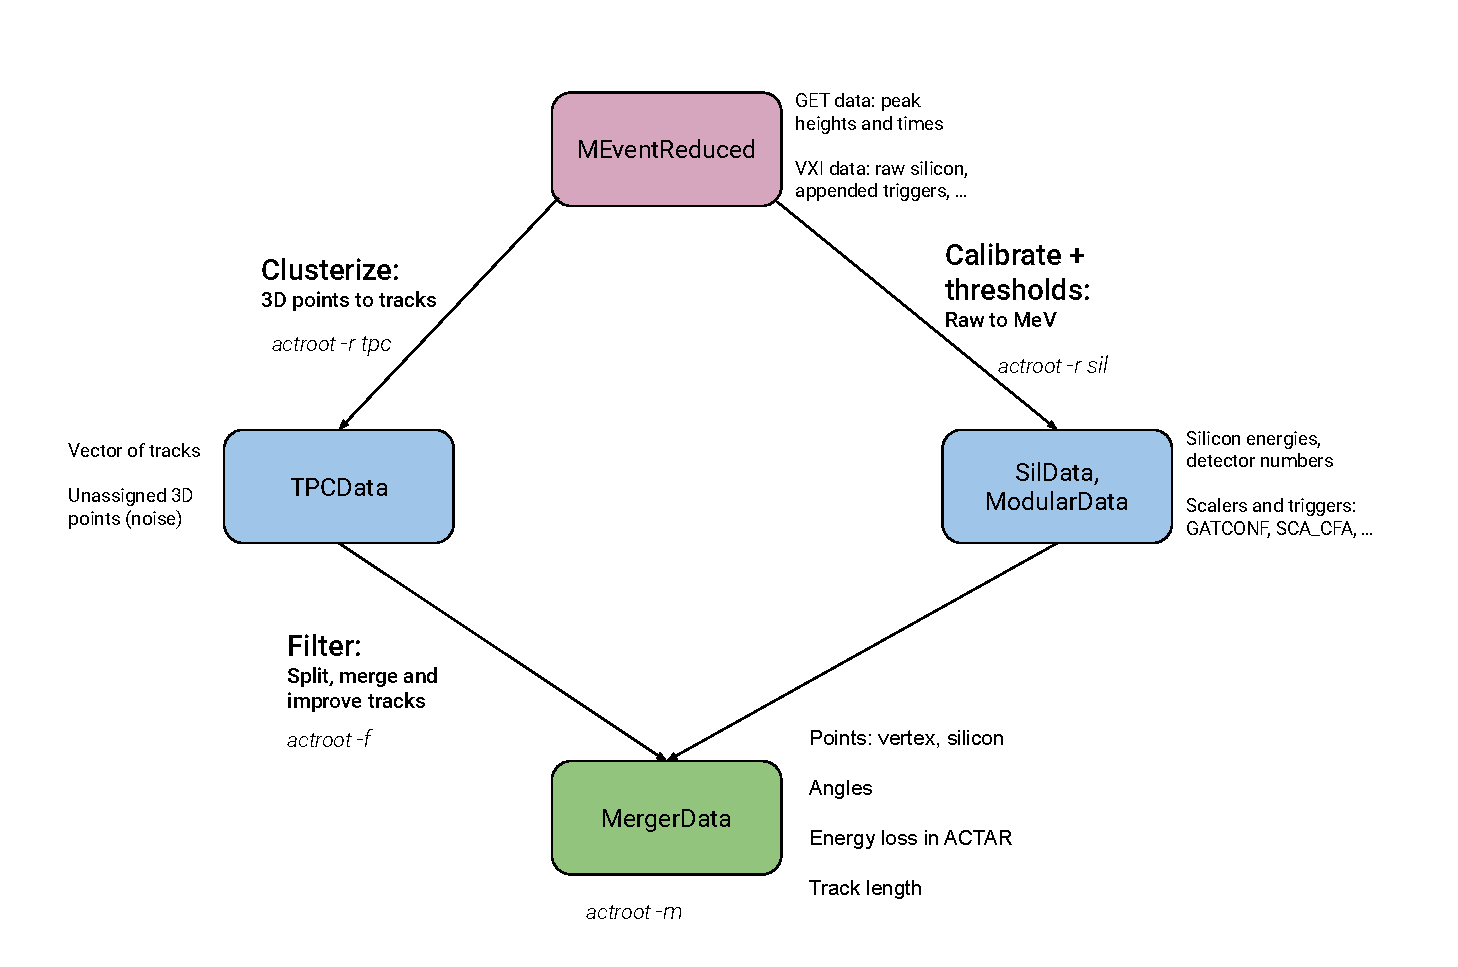
\includegraphics[width=0.9\linewidth]{Figures/ActRoot_schema.pdf}
	\caption{Actions tree of the analysis code.}
	\label{fig:scheme}
\end{figure}

A brief description of each element is presented in the following lines.
\begin{enumerate}
	\item \lstinline|MEventReduced|: minimal processed data. It merges the information from the pad plane (the GET 
	electronics) and the silicons (VXI), appending the external variables such as the scalers or triggers. This is our source data and it is further processed in two separate ways:
	\begin{itemize}
		\item \textbf{Cluster}: Handles the TPC data by merging the cloud of 3D points arising from the GET data to 
		form groups of points (\textit{clusters}) that indeed constitute \textbf{tracks}. 
		\item \textbf{Calibrate}: In charge of calibrating the silicon data and applying thresholds. It also reads the desired trigger variables.
	\end{itemize}
	\item \lstinline|TPCData|: Contains the vector of tracks result of the cluster process. It also stores points not assigned to any cluster. Afterwards:
	\begin{itemize}
		\item \textbf{Filter}: Complex action that transforms the vector of clusters to end up with only 2 or 3 that can be subsequently identified with the components of a \textbf{binary reaction}. Depending on the nature of the experiment, several actions might be needed to fulfill this goal: merging broken clusters, splitting artificially merged tracks, erasing noisy clusters (\textbf{contamination}, i.e., delta electrons), etc. 
	\end{itemize}
	\item \lstinline|SilData, ModularData|: Just a collection of silicon energies, detector index, and other useful data per event. By \textit{modular} we understand variables such as the \lstinline|GATCONF| (which unambiguously tells the detectors that triggered the acquisition) or the \lstinline|SCA_CFA| (that provides the number of beam particles in the CFA detector). Both classes do not require further processing. 
	\item \lstinline|MergerData|: Merges the three aforementioned classes to build a physical event. Given a set of conditions, it determines whether the event is good or not (provided the track or silicon multiplicity, the existence of a vertex, \lstinline|GATCONF| value, etc) and saves the following information:
	\begin{itemize}
		\item Angles of recoils with respect to the beam. 
		\item Energy at the silicon and the detector index.
		\item Average energy loss in the pad plane, which is of paramount importance for the PID.
		\item Track length. Also key to account for energy losses in the gas.
		\item The run and entry number, to unequivocally identify the event later.
		\item Other variables with debug purposes. 
	\end{itemize}
\end{enumerate}

One of the main goals of the code is to remain versatile: by using configuration files, the actions can be independently modified, permitting the analysis of different experiments without modifying the code. 
This is achieved by using a wide range of \textit{.conf} file, as follows:
\begin{itemize}
	\item \textit{detector.conf}: Configures general settings of the detectors: size of ACTAR pad plane, algorithms to be used, action files, and the merger conditions, so to speak.
	\item \textit{calibration.conf}: Calibrations to be used in the silicon energy conversion but also the look-up table for the pad plane (channel to <\textit{x}, \textit{y}>) and the gain matching parameters.
	\item Since there are different algorithms available to perform the \textit{Cluster} and \textit{Filter} actions, each of them reads a separate file:
	\begin{itemize}
		\item For the clustering: \textit{ransac.conf} or \textit{climb.conf}. Essentially, they set the minimum number of points to form a track.
		\item For the filtering: \textit{multiregion.conf} and \textit{multistep.conf}. This step is more complex. An attempt to explain these algorithms is given in \autoref{sec:2}.
	\end{itemize}
	The choice of algorithm is done in the \textit{detector.conf} file.
	\item \textit{data.conf}: Sets the vector of runs to analyze and the paths to read and store the \lstinline|.root| files.
\end{itemize}

All these files must lay under a \lstinline|configs/| directory in what will be called a \textbf{project} folder: the parent directory for all the analysis. It is in this folder that we can run the executables provided by the code, as noted in \autoref{fig:scheme} (\lstinline|actroot -flag OPTIONS|).

The goal of this manual is to provide a quick insight into the different algorithm settings for the \textit
{Filtering} part.

\section{Algorithms}\label{sec:2}
Two different types of algorithms to deal with voxels exist in the \textit{Algorithm} folder of \textit{ActRoot}:
\begin{itemize}
	\item Inheriting from \lstinline{VCluster}, they perform the basic clustering operation: joining voxels to form sets of voxels, i.e., clusters. Two have been implemented:
	      \begin{itemize}
		      \item \textbf{RANSAC}: randomly samples two points from the cloud to form a line. Points close to it by a given distance threshold constitute the cluster. The process is repeated $N$ times and only the \textit{best-ranked} clusters are kept.
		      \item \textbf{Climb}: clusters points based on the continuity principle: neighbor points \textit{should} belong to the same cluster. It was developed by J. Lois-Fuentes during his PhD \cite{lois23}, thus for more information see his thesis.
	      \end{itemize}
	      Both can be configured in the \verb|ransac.conf| or \verb|climb.conf| files, respectively.
	\item From \lstinline|VFilter|, this set of classes performs the treatment of the clusters, meaning this:
	      \begin{itemize}
		      \item Cleaning noise
		      \item Merging broken clusters
		      \item Splitting clusters
		      \item Finding the \textbf{reaction point}
		      \item Improving the quality of the line fits
	      \end{itemize}
	      Two are available now: \lstinline|MultiStep| and \lstinline|MultiRegion|. The former was employed for J. Lois experiment E796, while the latter is an \textit{easier} version.

	      Both leverage common functions that execute particular tasks. It is to this that we are going to explain in detail its workflow.
\end{itemize}

\subsection{Filtering algorithms}
Following the \lstinline|VFilter| class, the shared structure for all the filtering classes is:
\begin{enumerate}
	\item A pointer to the \lstinline|TPCData| has to be set by \lstinline|void VFilter::SetTPVData(TPCData* data)|
	\item The algorithm is executed by \lstinline|void VFilter::Run()|. This virtual function (i.e., mandatory to be implemented in any derived class) \textbf{sets the order of the inner functions}.
	\item Other methods are available depending on the derived class.
\end{enumerate}

\subsubsection{Common tasks}
There are a few steps that are usually needed by both classes. Hence, they are implemented in a \textit{global} fashion under \lstinline|ActAlgoFuncs.h,.cxx|.

These are:
\begin{itemize}
	\item \textbf{Merging similar clusters}: a cluster might be broken into smaller parts as a result of charge collection inefficacies or damaged pads. Therefore, it is essential to remerge them. This function iterates over the cluster vector and, by pairs, joins clusters if some conditions are met:
	      \begin{enumerate}
		      \item The distance between the central points of the two clusters is bellow \lstinline|MergeDistThresh|.
		      \item Both are quite parallel: their scalar product of fits is above \lstinline|MergeMinParallel| $\in [0, 1]$.
		      \item If 1 \textbf{and} 2 are met, the combined fit is done.
		      \item If, and only if, the $\chi^2_{new} \leq \textcolor{ProcessBlue}{\text{MergeChi2Factor}} \cdot \chi^2_{old}$, the larger cluster is merged into the smaller one and deleted. The scaling factor is usually $\sim \num{1.5}$.
	      \end{enumerate}
	\item \textbf{Compute a reaction point (RP) in 3D}: In general two lines in 3D do not perfectly intersect. On the contrary, the goal is to find the minimum approach distance and the two points on each line at which this occurs. 
	
	This function is schematically defined as:
	\begin{lstlisting}
		std::tuple<Point on A, Point on B, double min dist> 
		ComputeRPIn3D(Point A, Vector A, Point B, Vector B);
	\end{lstlisting}
	Specifying the points and the direction vectors of each line, one is given the two points and the distance between them. The RP is afterward calculated as the mean.
	\item \textbf{Cylinder cleaning} of a cluster: Some tracks may present \textit{transversal} anomalies that worsen the 3D linear fit. To delete them, a cylinder centered around the fit is defined and points outside it are tagged to be erased. This threshold, given by the radius of the cylinder, is known as \lstinline|CleanCylinderR|.
	
	Before deleting the voxels, a \textbf{check} is executed to determine whether the cluster will have enough remaining points. If not, it is kept unmodified. This threshold in the number of points is usually linked to the clustering algorithm by the function \lstinline|VCluster::GetMinPoints()|.

	\item \textbf{Separate recoil from beam}: In most reactions, there is a heavy recoil whose angle is so small that it remains undistinguishable from the beam particle. In these cases, the light particle is used to find the RP and, subsequently, this can be used to separate the beam from the secondary track. The procedure is as follows:
	\begin{enumerate}
		\item In the vector of clusters, find the \textbf{beam-like}.
		\item Split its voxels according to the X value: lower or greater than the RP.
		\item If enough voxels to form a new cluster (\lstinline|VFilter::GetMinPoints()|), erase.
		\item Refit the remaining cluster (and the new one if it is the case).
	\end{enumerate}
	The flag \lstinline|RPKeepSplit == false| allows to \textbf{delete} newly-formed cluster.
\end{itemize}



%\nocite{*}
\printbibliography
\end{document}